\documentclass[12pt]{article}
\usepackage{amsmath,amsfonts,graphicx,enumitem,amssymb,listings,graphicx,natbib}

\newcommand\E{\mathbb{E}}
\newcommand\R{\mathbf{R}}
\newcommand\SM{\mathbf{S}}
\newcommand\T{^\top}
\newcommand{\st}{\text{subject to }}
\newcommand{\ip}[2]{\langle #1, #2 \rangle}
\newcommand{\twomat}[4]{\begin{bmatrix} #1 & #2 \\ #3 & #4 \end{bmatrix}}
\newcommand{\tr}{\text{tr }}
\newcommand{\diag}{\text{diag}}
\newcommand{\knn}{\textit{k}NN}
\long\def\/*#1*/{}
\newenvironment{proof}{{\bf Proof:}}{\hfill\rule{2mm}{2mm}}

\usepackage{hyperref,enumerate}
\hypersetup{
    %colorlinks=true,
    %linkcolor=blue,
    %filecolor=magenta,
    %urlcolor=cyan,
}
\begin{document}
\title{Supervised Linear Distance Metric Learning with Convex Optimization \\ Convex and Nonsmooth Optimization Project\\CSCI-GA.2945.001 Spring 2018}
\author{Aodong Li\\NetID: al5350\\al5350@nyu.edu}
\date{May 14, 2018}
\maketitle

\begin{abstract}
In distance-based machine learning applications, different distance metrics (Euclidean distance v.s. distance along curved lines) capture the information of different interests, and thus can largely improve the model performance. Emerging as Mahalanobis distances, the distance metrics can be learned by different algorithms in various machine learning aspects. In particular, for this report, we take the path of convex optimizations over the space of positive semidefinite matrix. We start from the earliest work that applys convex optimization to this task and discuss its shortages; then present the main following work that makes effective advances on the earliest work by making up different deficiencies. Analysis and experiments demonstrate the deficiencies and show how other algorithms remedy the corresponding defects. Additional algorithmic derivations are also provided where the original paper omits. 
Investigations on the optimization techniques utilized by these papers illustrate that algorithms vary a lot based on the characteristics of the problem and an efficient design can be a piece of art.
We also compared the performance between the generic solver CVX and the original optimization algorithms provided by the papers.
\end{abstract}

\section{Introduction}
Distance metric learning serves as an important role in distance-based classification and clustering tasks in machine learning. Usually we need different distance metrics to measure the similarities of particular interests between two objects. For example, we are using k-means to cluster images of faces by pose and gender. Typically, it is hard to develop one optimal distance metric for both the pose task and the gender task.% even if, in both tasks, distances are computed between the same set of extracted features.

Motivated by these issues, different distance metrics for different tasks are quite desirable, where those tasks are specified by users. A conventional practice is to ask users to define which task that they are interested in. In particular, they provide the machine with two sets of pairs of data points -- an  equivalence set $S$ and an inequivalence set $D$. 
Pairs of data points $(x_i,x_j)$ in the equivalence set $S$ are thought to be similarly labeled and supposed to have small distances between them while $(x_i,x_j)$ in the inequivalence set $D$, considered to be differently labeled, should have large distances.
Both sets together define the constraints that                                                                                                                                                                                                                                                                                                                                                                                                                                                                                                                                                                                                                                                                                                                                                                                                                                                                                                                                           a desired distance metric is demanded to satisfy.  This intuition is first proposed by \citet{xing2003distance} and the two sets provided by users are termed as ``side information''. 

The side information can be used as supervised signals. These signals render the ability of utilizing supervised machine learning techniques to handle such problems, i.e., constructing an optimization problem and "learning" the metric by finding the optimal solution. 

Unlike the supervised learning behavior, \cite{yang2006distance} summarizes that unsupervised distance metric learning, or called manifold learning, focuses on learning an underlying low-dimensional manifold where geometric relationships between most of the observed data are preserved. This learned low-dimensional manifold is naturally related to dimension reduction techniques like Principle Component Analysis (PCA) and Laplacian Eigenmaps method (\cite{belkin2002laplacian}). These learning problems are usually solved by eigenvector methods based on second order statistics.

In this report, we will mainly focus on the important works on supervised metric learning and demonstrate the process of transforming the learning problem into a convex optimization problem. This report is organized as follows. Section 2 introduces the routemap that we will take and sums up the experience we obtain from this report. Section 3 presents some of the important distance metric learning algorithms that utilize convex optimization. Section 4 presents experiments  performed by the proposed optimization algorithms in the papers and the generic solver CVX. Section 5 concludes by summarizing the report.

\section{Routemap}

As we mentioned above, the very first work implementing distance metric learning via convex optimization comes from \cite{xing2003distance}. The learning problem is constructed as a semidefinite programming to find the optimal Mahalanobis distance.
The distance metric is parameterized by a positive semidefinite matrix $A$ that can be learned. 

Although \cite{xing2003distance} solved the problem from a totally new angle, several problems are still noticeable and many following work are come up with to deal with those defects. The first is that the number of parameters is almost quadratic in the number of features, %and there is no special structure of the problem 
and general solvers may scale poorly to large number of constraints and may be very inefficient. 
%So special optimization algorithms need to be specified. 
To deal with this, a probabilistic approach is proposed in \cite{yang2006efficient} to generalize the formulation to include a probabilistic view as well as to reduce the number of parameters by approximating the metric matrix with eigenvectors of the data covariance matrix.

On the other hand, the work proposed in \cite{xing2003distance} also suffers from the underlying assumption that clusters are generally modeled as normal or uni-modal distributions. The behavior of the global minimization of distances between all pairs of the similarly labeled points reflects this assumption. So the metric learned in this way is not appropriate to the multi-modal distributions like mixture models. A different objective for non-parametric models, such as \knn, is deserving. This extention is introduced by \cite{weinberger2009distance}, which is also formed as a semidefinite programming problem. 

Extending the boundaries of metric learning, \cite{shalev2004online} develops the online version and illustrates that it can be easily transformed into the batch version in a systematic way. These evolutions are presented in Figure \ref{evol}.
\begin{figure}[h]
\centering
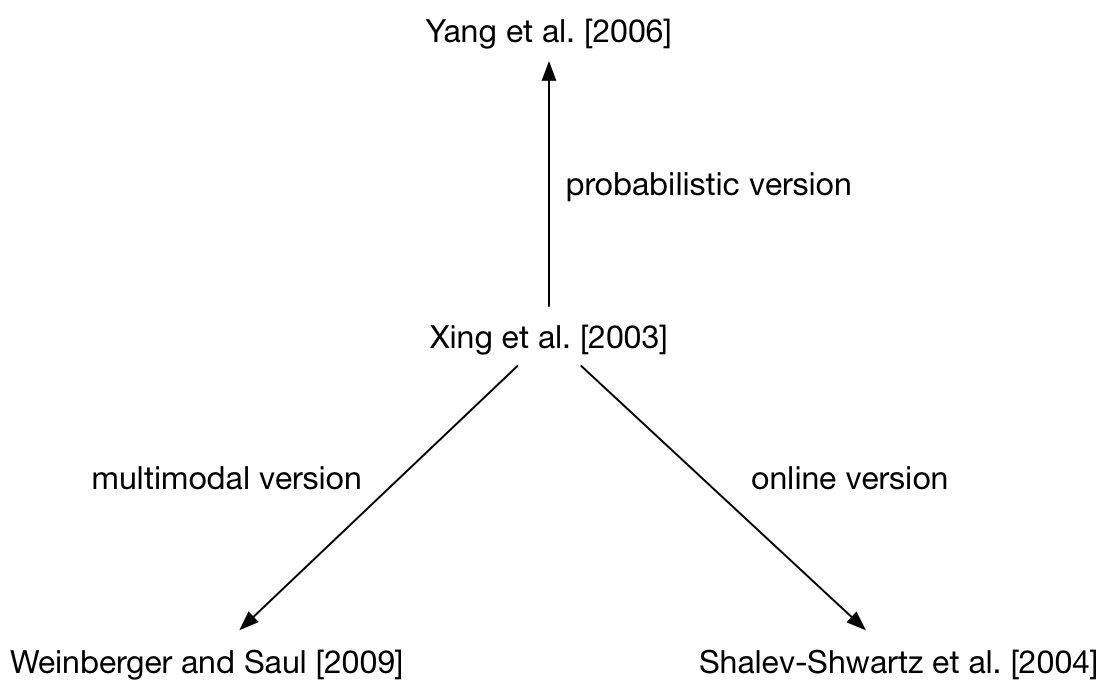
\includegraphics[width=10cm]{fig/evolution.jpg}
\caption{The main evolution of distance metric learning.}
\label{evol}
\end{figure}

By doing the resport, we realize that in practice, different problems usually assume different structures. Although sometimes general-purpose algorithms like interior-point methods can be utilized,  specific optimization method that takes advantage of the particular problem structure exhibits an easier implementation and better performance. To demonstrate this, we compare the specific optimization algorithms with the general solver CVX (\cite{grant2008cvx}) in section 4. 

Another explanation of why they did not use a free solver but paid large efforts to design one is that there did not exist such a  good solver like CVX  at that time. But, by investigating their original algorithms, we can see that all of these algorithms demonstrate systematic thoughts to construct and solve (smooth and nonsmooth) convex optimization problems. 
%(I think that's the reason resulting in a software like CVX.) 

We also notice that, which is another important point deserving attention, most of the constraint optimization problems (at least in distance metric learning) have a lot of equivalent forms and different forms may require different algorithms (e.g., LMNN's hard SDP optimization but easy sub-gradient descent methods). How to choose the appropriate problem form with the least expensive optimization algorithm may be another work of art.



\section{Distance Metric Learning}
In this section, we deliver three main methods for distance metric learning and their detailed derivations. In particular, we supplement the derivation details omitted by the authors. The three works represent respectively the global distance metric learning by \citet{xing2003distance}, the probabilistic version of global distance metric learning by \citet{yang2006efficient}, and the local distance metric learning by \citet{weinberger2009distance}.

We also analyse the original algorithms given by the papers and illustrate which optimization techniques they use to handle the optimization problem. It is quite interesting to see that in the era of lacking reliable generic solvers, the authors proposed quite concise and effective algorithms to deal with the optimization problem. These algorithms reflect the thoughts of interior-point methods and (sub)-gradient projection methods.

Before we get into the algorithmic details, we first present the background of distance metric learning.

\subsection{Background}
We begin by reviewing the definition of distance. A mapping $d:$ $\mathcal{X}\times\mathcal{X}\mapsto\R_+$ over a vector space $\mathcal{X}$ is called a metric or valid distance if for all vectors $\forall x_i, x_j, x_k\in \mathcal{X}$, it satisfies the properties:
\begin{itemize}[label={}]
\item[1.] $d(x_i,x_j) + d(x_j,x_k)\geq d(x_i,x_k)$ (triangular inequality).
\item[2.] $d(x_i,x_j)\geq 0$ (non-negativity).
\item[3.] $d(x_i,x_j) = d(x_j,x_i)$ (symmetry).
\item[4.] $d(x_i,x_j) = 0 \Longleftrightarrow x_i = x_j$ (distinguishability).
\end{itemize}

Strictly speaking, a mapping that satisfies the first three properties except the fourth is a pseudometric.

Given the definition, we can construct a valid pseudometric by setting \[d_L(x_i,x_j)=||L(x_i-x_j)||_2\] where $||\cdot||_2$ is $l2$ norm of a vector. The distance $d_L$ dictates that first apply a linear transformation on the vector $x$ by a real-valued linear map $L$, and then compute the Euclidean distance in the transformed space.

In particular we can rewrite $d_L$ as an equivalent pseudometric $d_A$ such that $d_A$ belongs to the family of Mahalanobis metrics,
\begin{align*}
d_L(x_i,x_j) & = ||L(x_i-x_j)||_2 \\
& = \sqrt{(L(x_i-x_j))\T(L(x_i-x_j))} \\
& = \sqrt{(x_i-x_j)\T L\T L(x_i-x_j)} \\
& = \sqrt{(x_i-x_j)\T A(x_i-x_j)} \\
& = d_A(x_i, x_j)
\end{align*}
where $A=L\T L$ is a symmetric positive semidefinite matrix. Note that  a positive definite matrix $A$ will define a valid metric.  We also denote $d_A(x_i, x_j)$ by $||x_i-x_j||_A$. To see why this is a valid pseudometric, we give a simplified proof.

\begin{proof}
The non-negativity is straightforward by the definition of positive semidefinite matrix. If $A\in\R^{n\times n}$ is positive semidefinite, then $\forall x\in \R^n$, \[x\T Ax\geq 0.\] Thus since $x_i-x_j\in \R^n$, $d_A(x_i,x_j)\geq 0$.

The symmetry is also straightforward. Because
\[(x_i-x_j)\T A(x_i-x_j) = (x_j-x_i)\T A(x_j-x_i),\] we have $d_A(x_i,x_j)=d_A(x_j,x_i)$.

To show the triangular inequality, we first derive a variant of Cauchy-Schwarz inequality. Given $x\neq 0$ and $y\neq 0$,
\begin{align*}
(x-\lambda y)\T A (x-\lambda y) &\geq 0 \quad(\text{for any $\lambda\in\R$})\\
x\T Ax + \lambda^2y\T Ay &\geq 2\lambda x\T Ay \\
x\T Ax + \frac{(x\T Ay)^2}{(y\T Ay)^2} y\T Ay &\geq \frac{2\cdot (x\T Ay)^2}{y\T Ay}\quad(\text{let $\lambda=\frac{x\T Ay}{y\T Ay}$}) \\
\sqrt{x\T Ax}\sqrt{y\T Ay}&\geq x\T Ay.
\end{align*}
Then we have the following inequality by using the above results,
\begin{align*}
(x+y)\T A(x+y)  & = x\T Ax + y\T Ay + 2x\T Ay \\
&\leq x\T Ax + y\T Ay + 2\sqrt{x\T Ax}\sqrt{y\T Ay} \\
& = (\sqrt{x\T Ax} + \sqrt{y\T Ay})^2.
\end{align*}
Setting $x = x_i-x_j$ and $y = x_j-x_k$ and plugging in, we have the triangular inequality $d(x_i,x_j) + d(x_j,x_k)\geq d(x_i,x_k)$.
\end{proof}

Now we have shown that Mahalanobis metrics are valid pseudometric, we can find such a metric either by the matrix $A$ or the matrix $L$ defined as above. Note that the matrix $L$ uniquely defines the matrix $A$, while the matrix $A$ defines $L$ up to some rotation (which preserves the distance anyway). Although we can explicitly solve the metric by $d_L$ without any constraints in the supervised setting, $d_A$ provides more benefits even with the constraint that $A$ has to be positive semidefinite. Because solving $d_A$ is usually equivalent to solving a convex optimization problem, the convexity avoids spurious local minimum and directly gives the global minimum! This property is quite desirable in local distance metric learning for multimodal distributions where locality might be prevalent.

\subsection{Global Distance Metric Learning for Clustering}
As described in section 1, when aided with the equivalence set $S$ and the inequivalence set $D$, we have an explicit goal that aims to minimize the distance for pairs $(x_i,x_j)\in S$ and maximize the distance for pairs $(x_i,x_j)\in D$. In other words, this shares a similar goal as Linear Discriminant Analysis (LDA): namely, to minimize the distances between data points with similar labels while maximize the distances between data points with different labels.  This similar goal with LDA might account for the similar behaviour with LDA (in the experiment section). It not only clusters the data but also tends to project them onto a line, which is the usual effect of LDA.

To exert such constraints, we simply add up all the distances in each set and constrain them with desired distances. The proposed optimization problem is as follows,
\begin{align}
\min_{A\in\SM_+^n} & \sum_{(x_i,x_j)\in S} (x_i-x_j)\T A(x_i-x_j)\label{obj1} \\
\st & \sum_{(x_i,x_j)\in D} \sqrt{(x_i-x_j)\T A(x_i-x_j)} \geq 1 \label{const1}\\
& A\succeq 0\label{const2}
\end{align}

It can be verified that both the objective function and constraints are convex, thus the constrained minimization is a convex optimization problem. Its solution ensures the global minimum. 

The choice of the constant 1 in the righthand side of (\ref{const1}) is arbitrary and not important. Changing it to any other positive constant $c$ results only in $A$ being scaled by $c^2$. In the experiments, we use this knowledge to enlarge our figure. It turns out such distance constraints are prevalent in the distance metric learning field and it usually assumes 1 than any other arbitrary values.

Another common question raised as to the optimization problem is that why use the square-root constraints instead of the simpler linear constraints. However, that linear constraint will always give a matrix $A$ with rank 1. The author did give some illustration in the paper, here we provide a complete one.  

\subsubsection{The Rayleigh Quotient}
The  Rayleigh Quotient assumes the form of 
\[\max_x \frac{x\T Ax}{x\T x}\]
where $A$ is symmetric. The  Rayleigh Quotient is prevalent in many machine learning applications since it usually provides an eigenvector solution of matrix $A$.

First notice that $\frac{x\T Ax}{x\T x} = \frac{{x'}\T Ax'}{{x'}\T x'}$ when we set $x' = cx$ for any $c\neq 0\in \R$, thus the problem may assume infinite solutions. So we might as well set constraints by solving the problem for $x$ with a unit norm $||x||_2^2=1$.

So the problem can be reformulated as 
\begin{align*}
\max_x\ & x\T Ax \\
\st & x\T x = 1.
\end{align*}

This problem can be readily solved by its KKT conditions or Lagrangian multipliers. The Lagrangian is 
\[L(x) = x\T Ax + \lambda(x\T x - 1)\] and its KKT conditions are 
\begin{align}
2Ax + 2\lambda x = 0 \\
x\T x  = 1
\end{align}

Hence the maximum is given when $Ax = -\lambda x$ where $-\lambda$ is an eigenvalue of $A$ and $x$ is its corresponding eigenvector. So the objective function is $x\T Ax = -\lambda x\T x = -\lambda$. The maximum is obtained at the eigenvector corresponding to the largest eigenvalue of $A$.

The generalized Rayleigh Quotient is \[\max_x \frac{x\T Ax}{x\T Bx}\] where $A$ and $B$ are both symmetric. Again, we choose a certain solution 
\begin{align*}
\max_x\ & x\T Ax \\
\st & x\T B x = 1.
\end{align*}

By similar argument, we can find that the solution is equivalent to
\begin{align}
2Ax + 2\lambda B x = 0 \\
x\T Bx  = 1
\end{align}
and the objective function is $x\T Ax = -\lambda x\T Bx = -\lambda$. The solution is the generalized eigenvector of the largest eigenvalue of $Ax=-\lambda Bx$.

Back to our convex optimization problem, if we replace the square root in \ref{const1} with a linear operator, it rings a bell to us for the Rayleigh Quatient-like quantity. And it turns out that $A$ is always of rank 1 because the optimization problem shares the similar solution with LDA, which is the solution of the Rayleigh Quotient. 

First note that we can rewrite the objective function and constraint function is a similar way with the Rayleigh Quotient,
\begin{align*}
\sum_{(x_i,x_j)\in T} (x_i-x_j)\T A(x_i-x_j) & = \sum_{(x_i,x_j)\in T} \tr((x_i-x_j)\T A(x_i-x_j)) \\
& = \sum_{(x_i,x_j)\in T} \tr( A(x_i-x_j)(x_i-x_j)\T) \\
& = \tr(A\sum_{(x_i,x_j)\in T}((x_i-x_j)(x_i-x_j)\T)) \\
& = \tr(AM_T) \\
& = \tr(\sum_{i=1}^n a_ia_i\T M_T ) \\
& = \sum_{i=1}^n a_i\T M_T a_i
%& = \langle A,M_S\rangle_F\quad(\text{$A$ is symmetric})
\end{align*}
where $M_T = \sum_{(x_i,x_j)\in T}(x_i-x_j)(x_i-x_j)\T$ and $A=\sum_{i=1}^n a_ia_i\T$ because $A\succeq 0$. 

We can reformulate the optimization problem as 
\begin{align*}
\min_{a_i\in\R^n} & \sum_{i=1}^n a_i\T M_S a_i \\
\st & \sum_{i=1}^n a_i\T M_D a_i \geq 1 \\
& \sum_{i=1}^n a_i a_i\T\succeq 0.
\end{align*}
Note that the last constraint is automatically satisfied. Similar argument gives the KKT conditions 
\begin{align*}
2M_Sa_i - 2\lambda M_Da_i = 0, \\
\lambda \geq 0,\ \sum_{i=1}^n a_i\T M_D a_i \geq 1,\\
\lambda(1- \sum_{i=1}^n a_i\T M_D a_i) = 0
\end{align*}
for all $a_i\in\R^n$.

Solving this system gives the solution for all $a_i$ to be the generalized eigenvector of the largest eigenvalue of $2M_Sa_i=\lambda M_Da_i$. Thus it makes the matrix $A=\sum_{i=1}^n a_i a_i\T$ to be rank 1.

\subsubsection{The case of diagonal A}
In this section and the next one, we begin to analyse the original algorithm given by the paper and illustrate which techniques it uses to handle the optimization problem. It is quite interesting to see that in the era of lacking reliable generic solvers, the authors proposed quite concise algorithms to deal with the optimization problem. These algorithms reflect the thoughts of interior-point methods.

For this case, the author proposed a barrier-like method and use Newton's method to solve the problem. Since $A$ is diagonal, there are only $n$ parameters to be specified which makes it possible to efficiently compute the Hessian and its inverse. The author eliminates the constraint (\ref{const1}) by putting it into a $\log$ function and subtracting it from the objective function, which essentially imitates the barrier methods, although it explicitly sets the barrier parameter $t$ to be 1 ($t$ usually increases from iterations to iterations in barrier methods). To make sure $A\succeq 0$, during each iteration of the Newton's method, it employs a line search to limit the step size such that $A^{(k)}\succeq 0$ for step $k$. This is also the essence of interior-point methods.

In particular, the following objective function is optimized,
\begin{align*}
 g(A) =  \sum_{(x_i,x_j)\in S} (x_i-x_j)\T A(x_i-x_j) -\log\left(\sum_{(x_i,x_j)\in D} \sqrt{(x_i-x_j)\T A(x_i-x_j)}\right)
\end{align*}
and minimizing $g$ is equivalent, up to a multiplication of $A$ by a positive constant (because the constant in (\ref{const1}) is arbitrary), to solve the original optimization problem.


\subsubsection{The case of full A}

If we use a full symmetric matrix $A$, the number of parameters that need to be solved is $O(n^2)$. And the Newton's method becomes quite expensive because the inverse operation requires $O(n^3)$ even after being optimized. Thus instead of utilizing Newton's method, the author proposed a gradient ascent method with iterative projection algorithm. 

The experience we get here is that for problems with large number of parameters, we had better to use gradient methods to avoid computing the inverse of the Hessian matrix. The algorithms applying the Quasi-Newton methods are also worth a try.

In particular, to facilitate the computation, the author exchanges the constraints and objectives,
\begin{align}
\max_{A\in\SM_+^n} & \sum_{(x_i,x_j)\in D} \sqrt{(x_i-x_j)\T A(x_i-x_j)}\\
\st &   \sum_{(x_i,x_j)\in S} (x_i-x_j)\T A(x_i-x_j)\leq 1 \label{cconst1}\\
& A\succeq 0\label{cconst2}
\end{align}
Every time update $A$ by gradient ascent, and make sure projecting the new value onto the convex domain of the contraints. The projection is executed as iterations until convergence,
\[A := {\arg\min}_{A'}\{||A'-A||_F^2: A'\in C\}.\]

For constraint (\ref{cconst1}), this projection can be seen as a quadratic programming and can be solved by alternating projections in $O(n^2)$ time. In essence, alternating projection algorithms provably converge (\citet{vandenberghe1996semidefinite}). For constraint (\ref{cconst2}), it can be solved by eigen-decomposition of $A = V\Sigma V\T$ and change the eigenvalues $\Sigma'=\max(0,\Sigma)$ thus $A'=V\Sigma' V\T$ is positive semidefinite.

In conclusion, the whole purpose is to find the direction (by Newton's method or gradient ascent) to the maximum as well as keep the solution satisfying the constraints (by projection).

\subsection{Probabilistic Global Distance Metric Learning}

It can be seen that the number of parameters in the optimization problem (\ref{obj1})-(\ref{const2}) is $O(n^2)$ where $n$ is the number of dimensions of the data. And the optimization algorithm is kind of tricky to come up with. Instead, \citet{yang2006distance} provides an approximate on the metric matrix $A$. In particular, they first compute the covariance matrix $M$ of all the data, 
\[M = \frac{1}{n}\sum_{i=1}^{n}x_ix_i\T,\]
which include the pairwise correlation between any two features. Further more, if we use the design matrix $X$ which has each data point at each row, then $M=X\T X$ up to a constant $n$. Denote the top $K$ eigenvectors of $M$ by $\{v_i\}_{i=1}^K$. Then they assume that $A$ is a linear combination of the top $K$ eigenvectors
\[A=\sum_{i=1}^{K} \gamma_iv_iv_i\T,\quad \gamma_i\geq0.\]

In the paper, they did not give the reason why they take $A$ in this form. But I think they might refer to the results of unsupervised distance metric learning which usually gives the eigenvector solution, and they use the results here as a kind of approximation. Furthermore, such an approximation can also be used for the original programming to reduce the number of parameters. We leave this as a future work.

Given this kind of approximation, they assume a logistic regression model to estimate the probability of any two data points sharing the same class, i.e.,
\begin{align*}
P(y_{i,j}|x_i,x_j)&=\frac{1}{1+\exp(-y_{i,j}(||x_i-x_j||_A^2 - \mu))} \\
& = \frac{1}{1+\exp(-y_{i,j}(\sum_{k=1}^K\gamma_kw^k_{i,j} - \mu))} 
\end{align*}
where 
\begin{align*}
y_{i,j} &= \left\{
\begin{array}{ll}
1, & (x_i,x_j)\in S,\\
-1, & (x_i,x_j)\in D.
\end{array}\right.
\\
w^k_{i,j}& = (x_i-x_j)\T v_kv_k\T (x_i-x_j).
\end{align*}

This is a probabilistic model, and if we assume that each data is generated iid, then we can estimate the parameters by maximum likelihood. In particular, the log-likelihood function is
\begin{align*}
L(\{v_i\}_{i=1}^K)  =& -\sum_{(x_i,x_j)\in S}\log\left(1+\exp\left(-\sum_{k=1}^K\gamma_kw^k_{i,j} + \mu\right)\right) \\
& - \sum_{(x_i,x_j)\in D}\log\left(1+\exp\left(\sum_{k=1}^K\gamma_kw^k_{i,j} - \mu\right)\right)
\end{align*}
and the convex problem is 
\begin{align*}
\min\ & L(\{v_i\}_{i=1}^K)\\
\st & \mu\geq 0, \gamma_i\geq 0,i=1,...,K.
\end{align*}
This problem can be solved directly using Newton's method or gradient descent method. Notice that during the iterations make sure that the constraints are valid by projection. This formulation spares the efforts of designing efficient algorithms.




\subsection{Local Distance Metric Learning for Classification}
The optimization problem (\ref{obj1})-(\ref{const2}) is designed for clustering. In these algorithms, clusters are generally modeled as normal or unimodel distributions. To see this, note that the objective function and the constraints are exerted on all pairs of the similarly labeled data and differently labeled data. It does not take local clusters into consideration. For this reason, however, global distance metric is not appropriate for multimodal data distributions, neither in clustering nor in classification.

A representative work to extend this into the local distance metric learning comes from \citet{weinberger2009distance}. The algorithm is referred to as Large Margin Nearest Neighbor (LMNN). It realizes its power with the non-parametric benefits of \knn\  algorithm. In addition to formulate a convex optimization problem, they attempt to maximize the margin of which the model correctly classifies labeled data points in the training set.

Based on the main intuitions that 1) neighbors should share similarly labels and should be as close as possible, and that 2) data with differently labels should be separated as far as possible, the authors formulated the objective function and minimize it:
\begin{multline}
f(A) = (1-\mu)\sum_{i,j\in\text{Neighbor}(i)}||x_i-x_j||_A^2 \\+ \mu\sum_{i,j\in\text{Neighbor}(i),l}(1-y_{il})\left[1+||x_i-x_j||_A^2-||x_i-x_l||_A^2\right]_+
\label{obj_l}
\end{multline}
where $y_{il}=1$ if and only if $y_i = y_l$ and $y_{il}=0$ otherwise, and $[\cdot]_+=\max(0,\cdot)$ represents the hinge loss. $\mu$ is the hyperparameter that controls the weight of each term, usually taken to be $0.5$. $\text{Neighbor}(i)$ is the set of data that share the same label with $x_i$.

This objective function is the most important thing and deserves to take a closer look. The first term is as normal to the traditional term we have seen above, it dictates that neighbors should get close. But the second term is a little different, it demands maximizing soft-margin like support vector machine (SVM) does. This soft-margin is triggered by a hinge loss. Here the authors defined such a loss as that is triggered when a differently labeled data $x_l$ approaches into the neighborhood of $x_i$, where the neighborhood is imposed by the similarly labeled neighbors of $x_i$. Thus, the loss for two differently labeled data $x_i$ and $x_j$ appears when the following condition happens:
\[||x_i-x_l||_A^2\leq ||x_i-x_j||_A^2 + 1, \quad x_j\in\text{Neighbor}(i)\]
and the loss is 0 otherwise.

Formally the hinge loss when we are considering the point $x_i$ is
\[\sum_{i,j\in\text{Neighbor}(i),l}(1-y_{il})\left[1+||x_i-x_j||_A^2-||x_i-x_l||_A^2\right]_+\]
which is the second term of the objective function.

We can therefore construct an optimization problem. The hinge loss used in the functions automatically trigger non-differentiable objectives. This can be either reformulated into SDP framework by introducing slackness variables or solved directly using sub-gradient descent methods. 

Now first consider the SDP framework. Notice that the second term in (\ref{obj_l}) is a piecewise linear function of $A$. Typically we deal with piecewise linear functions by introducing a slack variable $t$ and the final optimization problem is an SDP which is consistently linear of $A$:
\begin{align}
\min\ &(1-\mu)\sum_{i,j\in\text{Neighbor}(i)}||x_i-x_j||_A^2 + \mu\sum_{i,j\in\text{Neighbor}(i),l}(1-y_{il})t_{ijl} \label{ldmobj_1}\\
\st & t_{ijl} \geq 1+||x_i-x_j||_A^2-||x_i-x_l||_A^2 \\
& t_{ijl} \geq 0 \\
& A\succeq 0 \label{ldmconst_3}
\end{align}

One of the big problem is that the number of constraints is quite large so that a general-purpose solver like CVX tends to scale poorly. Thus the authors implement their special-purpose solver, exploiting the sparsity of the structure, i.e., that most of the slack variables are 0 because the number of data points that can trigger a loss defined above is quite small. This fact coincides with the complementary slackness of strong duality, which is also formulated  in SVM literature. Thus, very few active constraints in the SDP can greatly speed up the solving process by only monitoring a fraction of the margin constraints. 
%We refer the interested readers to the details in the paper (\citet{weinberger2009distance}).

So rather than solving the SDP optimization problems (\ref{ldmobj_1}) - (\ref{ldmconst_3}), the new solver directly solves the objective (\ref{obj_l}) using sub-gradient descent methods (\cite{boyd2003subgradient}). Then a projection is made to ensure that $A$ is updated within the positive semidefinite cone after each step. Again, the projection algorithms provably converge (\citet{vandenberghe1996semidefinite}). Almost all the algorithms trying to achieve large margin (involving piecewise linear hinge loss) can utilize the sub-gradient methods. These methods converge to the correct solution, provided that the gradient step-size is sufficiently small (\cite{boyd2003subgradient}).

Recently, the authors used the squared LMNN loss (which is differentiable) and developed new solvers by using limited memory BFGS algorithm (\cite{liu1989limited}), which is an efficient and effective algorithm for nonconvex and smooth optimization. This further improves the performance.




\section{Experiments}\footnote{The code list can be found at https://github.com/stamdlee/DistanceMetricLearning}
In this section, we implement algorithms on cluster tasks with side information where the side information is given as class signals. We implement both the original algorithms (\citet{xing2003distance}) and the CVX version on global distance metric learning. For the local distance metric learning, we use LMNN (\citet{weinberger2009distance}). Experiments demonstrate that the unimodal assumption of the global distance metric learning and that this drawback is conquered by local distance metric learning.

\subsection{Global Distance Metric Learning}

We generate artificial data for this section and provide analysis on the optimization problem. Here we use two Gaussian clusters as two different classes. Cluster 1 is sampled from $\mathcal{N}(x|\pi_1, \Sigma^{-1}_1)$ and cluster 2 is sampled from $\mathcal{N}(x|\pi_2, \Sigma^{-1}_2)$ where
\begin{align*}
\pi_1 = (5,5)\T,\quad\Sigma_1=\twomat{1}{0}{0}{1},\\
\pi_2 = (10,10)\T,\quad\Sigma_2=\twomat{2}{0}{0}{2}.
\end{align*}
20 samples for each cluster are illustrated at Figure \ref{fig1}. Note that the data has been normalized.
\begin{figure}[h]
\centering
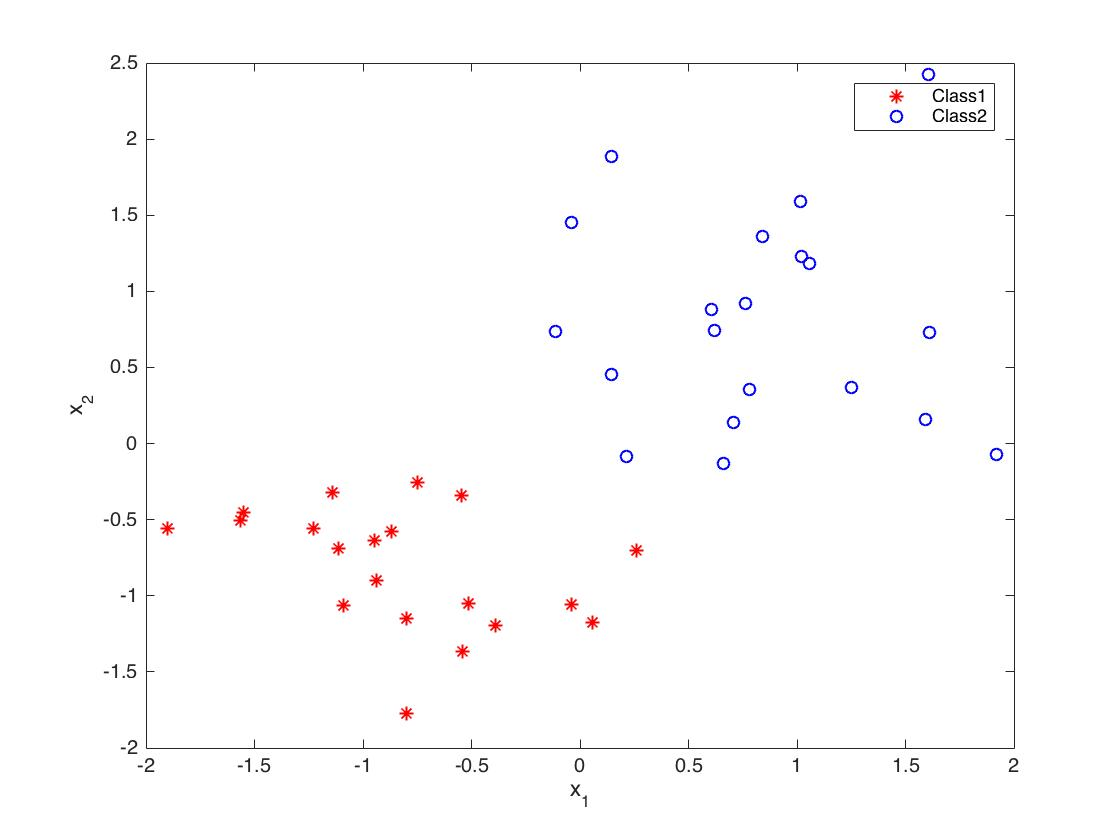
\includegraphics[width=10cm]{fig/data.jpg}
\caption{Artificial data illustration.}
\label{fig1}
\end{figure}

First we solve this convex optimization problem by CVX. Depending on whether we learn a diagonal or full $A$, we obtain
\begin{align*}
 A_{diagonal}^{cvx} = \twomat{0.2008}{0}{0}{0.9129}; 
 A_{full}^{cvx} = \twomat{ 0.8044 }{0.5831}{0.5831}{0.5570}.
\end{align*}

And the transformed data $A^{\frac{1}{2}}x$ is plotted in Figure \ref{fig2}. Here we use 40 pairs in each set, i.e., the equivalence set $S$ and the inequivalence set $D$. It can be seen that the data is clustered as expected. The left figure is for diagonal distance matrix and the right figure is for full matrix. When we use the full distance metric matrix, the transformed cluster tends to lie on a line. This behavior, as illustrated in section 3.2.1, might come from the similar solution with LDA.
\begin{figure}[h]
\centering
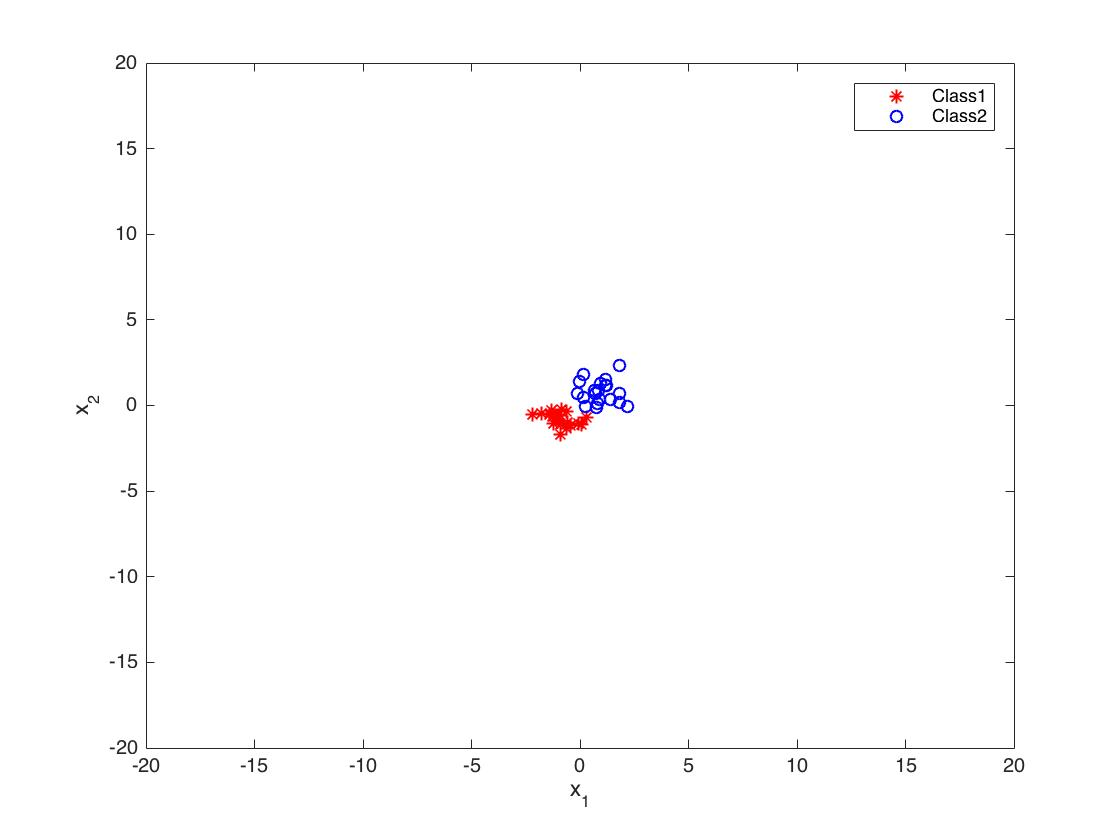
\includegraphics[width=6.5cm]{fig/diagA_2.jpg}
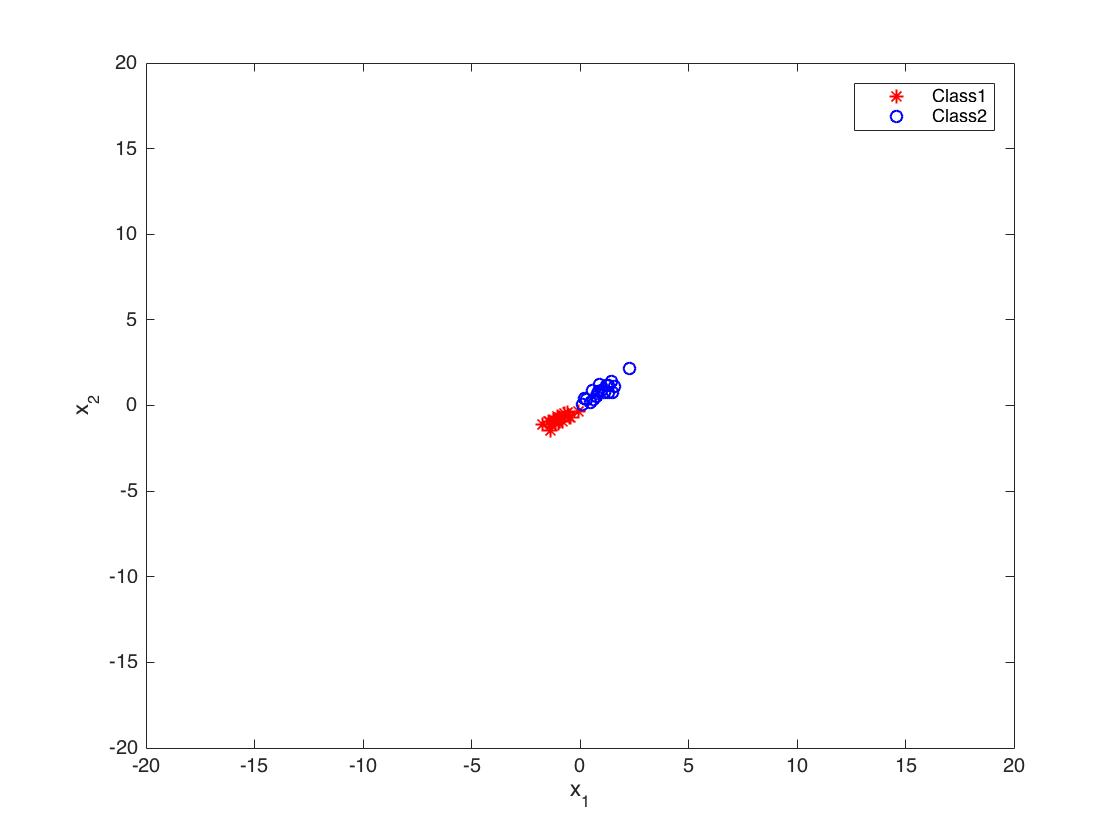
\includegraphics[width=6.5cm]{fig/fullA_2.jpg}
\caption{Transformed artificial data illustration. The left one is for diagonal transformation matrix and the right one is for full transformation matrix.}
\label{fig2}
\end{figure}

If we use the algorithm provided by the paper, that is, kind of like the barrier methods, also gives an approximate solution. Depending on whether we learn a diagonal or full $A$, we obtain
\begin{align*}
 A_{diagonal}^{ori} = \twomat{0.0598}{0}{0}{0.0121}; 
 A_{full}^{ori} = \twomat{0.0302}{0.0246}{0.0246}{0.0201}.
\end{align*}

It can be seen that the solutions produced by CVX and the ones produced by the original algorithms are approximately proportional. This is acceptable since different scales only result in different ``margins''. But the speeds are quite different. Here we use artificial data to illustrate the speed difference (refer to Table \ref{table1} and Table \ref{table2}). It shows that the original diagonal matrix solver is quite fast but not stable. Sometimes the iteration step cannot be computed. Also, the original full matrix solver is fast when the condition is good and well-suited for computation, but quite slow if in bad condition. In contrast, the generic solver CVX is much more stable and there is not much difference between  different matrix structures. Its performance only correlates to the matrix dimension.

\begin{table}[h]
\centering
 \begin{tabular}{ c|c|c }
solvers & d = 2, \#constraint = 40 & d = 2, \#constraint = 200  \\ \hline\hline
original diag & 0.085s  &  N/A\\
original full & 0.062s & 0.082s\\
cvx diag & 2.318s & 7.669s  \\
cvx full  & 2.175s& 6.958s \\
\end{tabular}
\caption{Elapsed time for different solvers (i).}
\label{table1}
\end{table}
\begin{table}[h]
\centering
\begin{tabular}{ c|c|c }
solvers &  d = 10, \#constraint = 40 & d = 10, \#constraint = 200 \\\hline\hline
original diag & 0.012s & 0.048s\\
original full & 11.963s & 5.708s\\
cvx diag & 2.120s & 7.213s \\
cvx full  & 2.369s & 7.620s \\
\end{tabular}
\caption{Elapsed time for different solvers (ii).}
\label{table2}
\end{table}


\begin{figure}[h!]
\centering
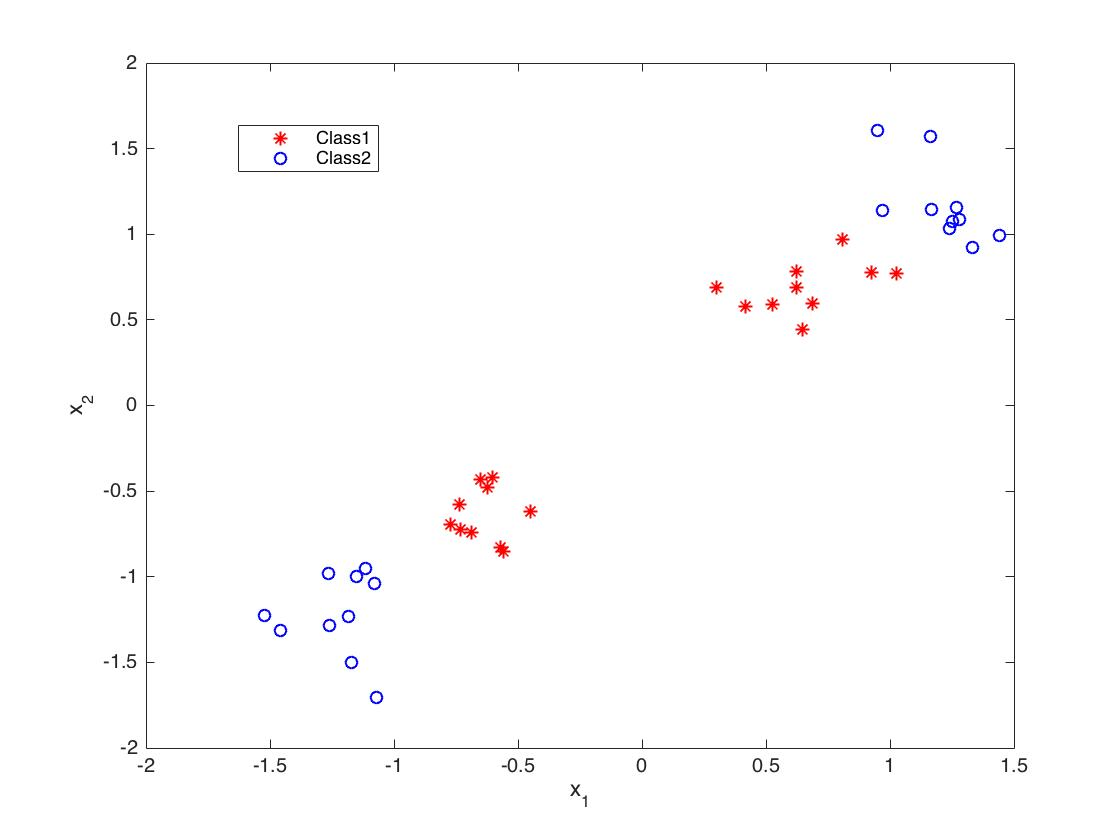
\includegraphics[width=6.5cm]{fig/mult-dat.jpg}
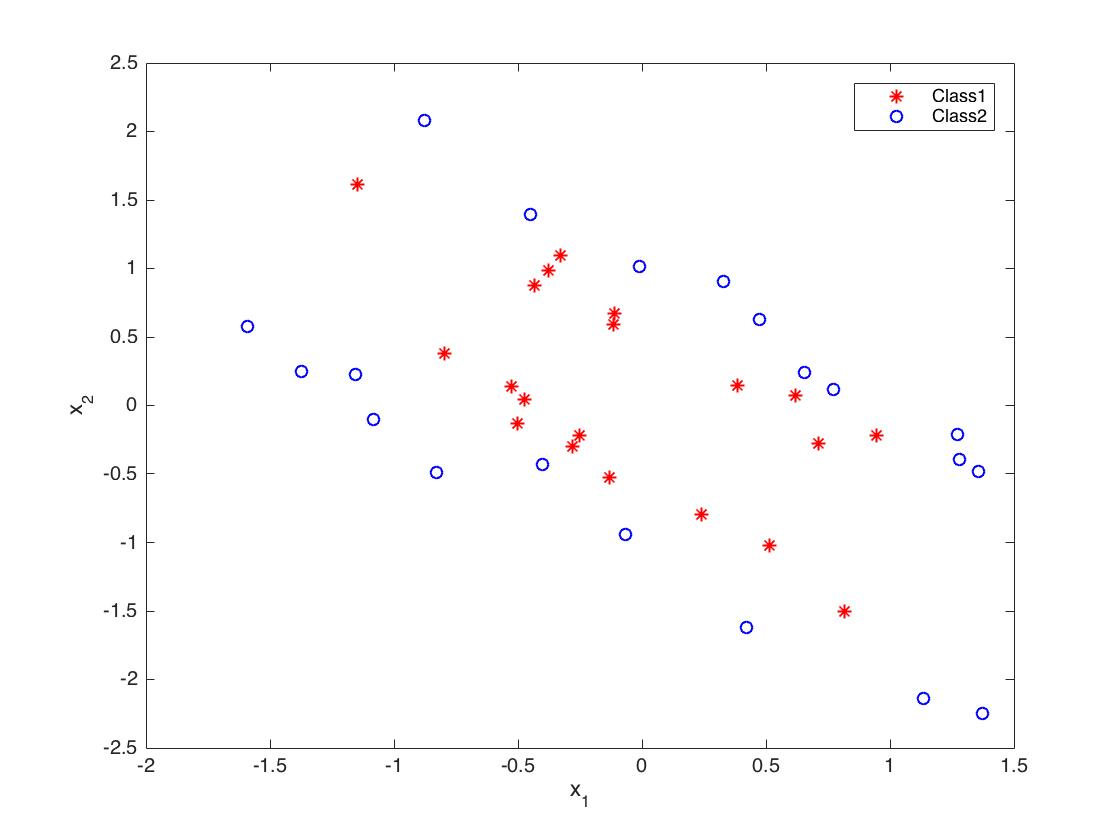
\includegraphics[width=6.5cm]{fig/mult-projected.jpg}
\caption{Multimodal data illustration. The left is the original data and the right is transformed data by a full matrix $A$.}
\label{fig3}
\end{figure}




Here we also give an illustration of the global nature of this metric. As we mentioned in section 3.4, the objective function and the constraints  (\ref{obj1}) -- (\ref{const2})  are exerted on all pairs of the similarly labeled data and differently labeled data. It essentially assumes that the distribution is unimodal or normal. We give a multimodal distribution data in Figure \ref{fig3}, which is a mixture of Gaussian composed of two mixtures for each class. The corresponding transformed data by a full matrix is also given in Figure \ref{fig3}. It can be seen that the learned distance metric collapses the data and makes things worse by dragging close different classes. Fortunately, this problem is fixed by local distance metric learning algorithm, e.g., LMNN.


\subsection{Local Distance Metric Learning}

\begin{figure}[h!]
\centering
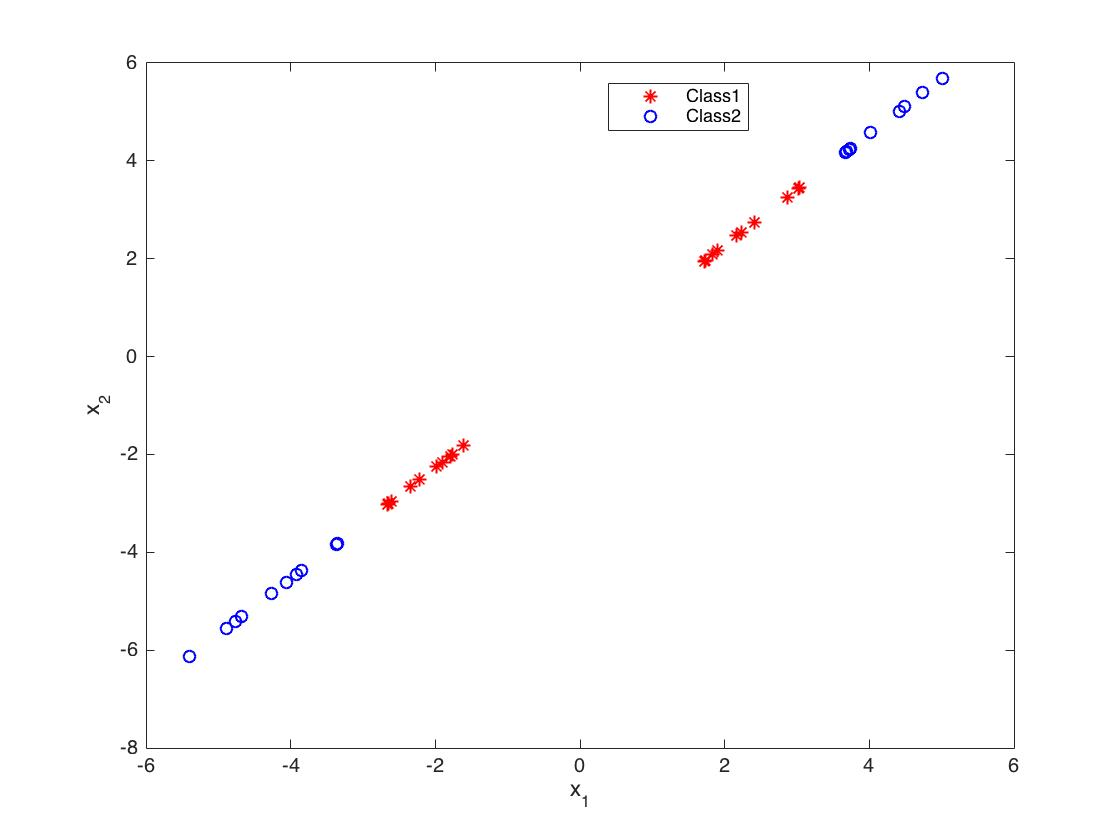
\includegraphics[width=10cm]{fig/mult-lmnn.jpg}
\caption{Multimodal transformed data by LMNN algorithm.}
\label{fig4}
\end{figure}


Now we apply local distance metric learning algorithm LMNN algorithm to the same multimodal dataset and set $K=1$, which indicates a nearest neighbor. Figure \ref{fig4} shows that things are getting better and the clusters are preserved by projecting onto a line. This line-like projection behavior is similar to the global distance metric learning algorithm we used above.


\section{Conclusion}
In this report, we focus on the subject of distance metric learning. Although this subject covers a broad field, we particularly survey its supervised linear forms and omit the unsupervised or more sophisticated non-linear forms. Despite the relatively simple form, such learning problems dictate quite smart formulation of convex optimization programmings, especially, SDPs. Interestingly, however, the authors are reluctant to use the general solver but try to come up with the specific optimization algorithms by taking advantage of the particular structure. These special-purpose algorithms more or less reflect the idea of most techniques in convex optimization, such as barrier methods, alternating projection, sub-gradient descent methods et al. In general,  the final goal is to find the direction (by Newton's method or gradient ascent/descent) to the maximum/minimum as well as keep the solution satisfying the constraints (by projection). Another important point deserving notice is that most of the constraint optimization problems (at least in distance metric learning) have a lot of equivalent forms and different forms may require different algorithms (e.g., LMNN's SDP optimization and sub-gradient descent methods). The performance varies from algorithm to algorithm, thus choosing an appropriate problem form with the least-cost  optimization algorithm is also an important task. For the experiments, we implement two main algorithms and illustrate one's drawback is fixed by the other.




\bibliographystyle{plainnat}
\bibliography{ref.bib}

\end{document}
